\begin{flushleft}
	\section{\textcolor{cyan}{Matérial et outillage: }}
		\subsection{\textcolor{green}{NodeMcu (ESP8266) :}}
		ESP8266 est le nom d’un tristement célèbre module WiFi qui est un système sur puce (SoC) développé par Espressif Systems, une société basée à Shanghai. Utilisé à l’origine avec les cartes Arduino pour les projets matériels compatibles WiFi, il est rapidement devenu une carte de développement autonome bon marché compatible Arduino. Il peut fonctionner en toute autonomie, sans microcontrôleur supplémentaire comme la carte Arduino par exemple.\newline
		
		Domotique et IOT – connecter des appareils à un réseau est une grande tendance en constante évolution de nos jours. Compte tenu de son prix bon marché, de sa configuration conviviale et de son énorme communauté qui contribue aux bibliothèques et aux projets open source, vous comprendrez immédiatement pourquoi cette puce suscite autant d’intérêt.\newline
		
		Ce microcontrôleur (MCU) peut être utilisé pour contrôler et surveiller des systèmes et des produits d’ingénierie, l’enregistrement des données des capteurs et plus encore. Tout cela en fait le matériel idéal pour les projets de domotique connectée. Il se présente sous de nombreuses formes, la NodeMcu (avec la dernière puce ESP8266-E12) étant la carte de développement la plus populaire d’entre elles. Image : La carte de développement NodeMcu est la variante ESP8266 la plus populaire.\newline
		\begin{figure}[h]
			\centering
			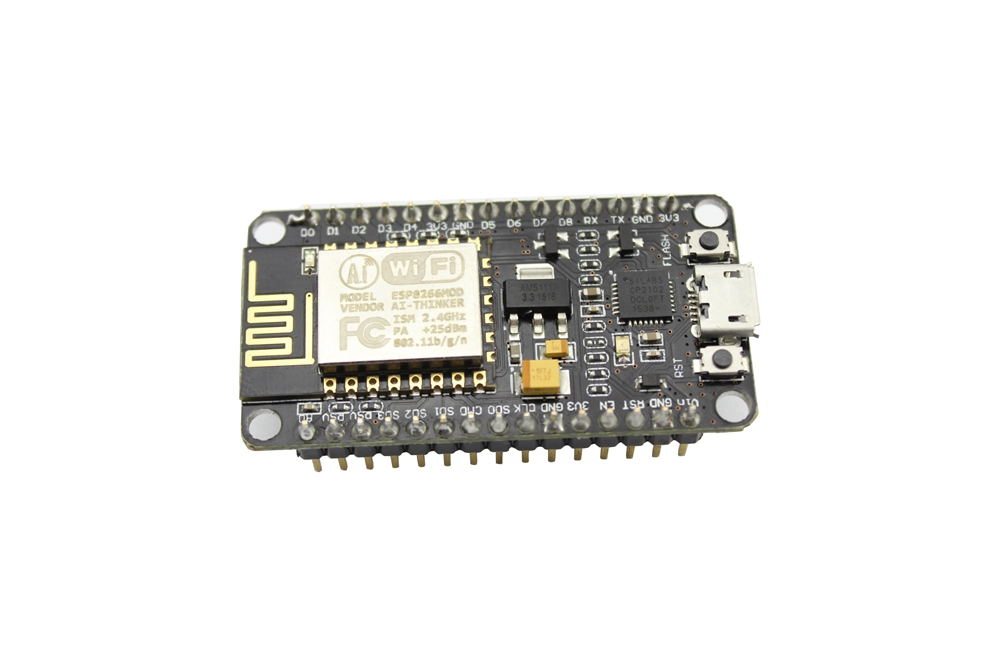
\includegraphics{chapitres/images/NodeMcu.jpg}
			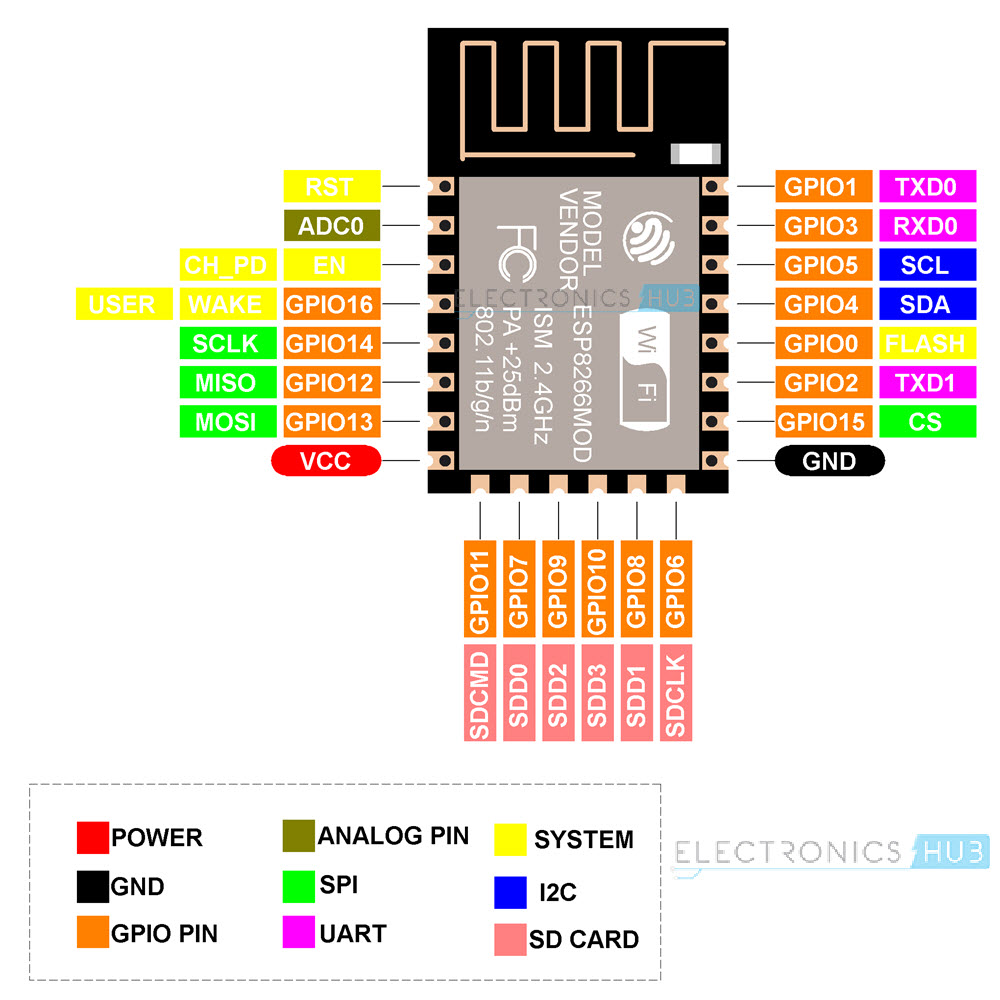
\includegraphics{chapitres/images/ESP8266_12X.jpg}
			\caption{NodeMcu ou ESP8266}
			\label{fig:labelname}
		\end{figure}
		Toutes les variantes de l’ESP8266 disposent d’un processeur principal ESP8266EX et d’un microcontrôleur Tensilica L106 32 bits. Il s’agit d’un SoC (System-On-Chip) à faible coût, haute performance, faible consommation d’énergie, facile à programmer, sans fil. Il fournit des capacités pour le Wi-Fi 2,4 GHz (802.11 b / g / n, prenant en charge WPA / WPA2), l’entrée / sortie à usage général (13 GPIO), le circuit inter-intégré (I²C), la conversion analogique-numérique (CAN 10 bits), l’interface périphérique série (SPI), les interfaces I²S avec DMA (partage de broches avec GPIO), UART (sur des broches dédiées, plus un UART en transmission seule peut être activé sur GPIO2) et la modulation de largeur d’impulsion (PWM).\newline
		
		Il dispose d’un programmateur intégré et d’un régulateur de tension, qui permettent de clignoter et d’alimenter l’appareil via micro-USB. Le système fonctionne à 3,3 V.\newpage
	
		\subsection{\textcolor{green}{Oxymètre de pouls MAX30102 :}}
			\begin{figure}[h]
			\centering
			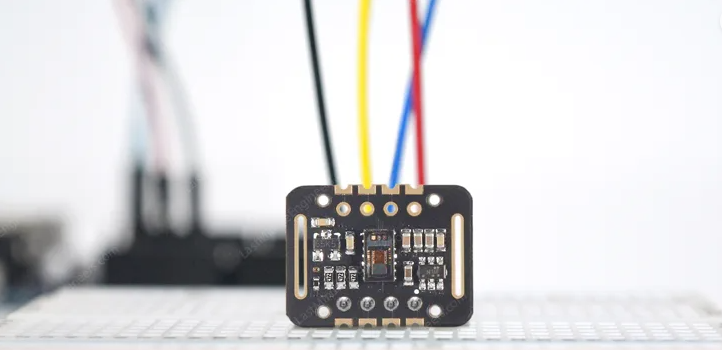
\includegraphics{chapitres/images/Capteur1.PNG}
			\caption{L’oxymètre de pouls et capteur de fréquence cardiaque MAX30102}
			\label{fig:labelname}
			\end{figure}
		L’oxymètre de pouls et capteur de fréquence cardiaque MAX30102 est un capteur biométrique plug-and-play basse consommation basé sur I2C. Il peut être utilisé par les étudiants, les amateurs, les ingénieurs, les fabricants et les développeurs de jeux et mobiles qui souhaitent intégrer des données de fréquence cardiaque en direct dans leurs projets.\newline
		
		\begin{itemize}
			\item {\Large  Présentation matérielle du module MAX30102}
		\end{itemize}
		Le module est équipé du MAX30102 – un circuit intégré moderne (successeur du MAX30100) et d’oxymètre de pouls et de capteur de fréquence cardiaque d’Analog Devices. Il combine deux LED, un photodétecteur, une optique optimisée et un traitement du signal analogique à faible bruit pour détecter les signaux d’oxymétrie de pouls (SpO2) et de fréquence cardiaque (HR).
		\begin{figure}[h]
			\centering
			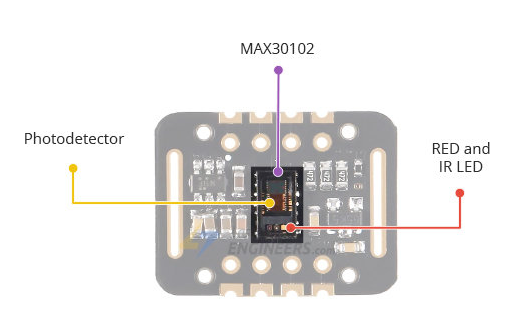
\includegraphics{chapitres/images/Capteur2.PNG}
			\label{fig:labelname}
		\end{figure}
		
		Derrière la fenêtre d’un côté, le MAX30102 dispose de deux LED – une LED ROUGE et une LED IR. De l’autre côté se trouve un photodétecteur très sensible. L’idée est que vous faites briller une seule LED à la fois, détectant la quantité de lumière qui rallume sur le détecteur, et, en fonction de la signature, vous pouvez mesurer le niveau d’oxygène dans le sang et la fréquence cardiaque.\newline
		\newpage
	\begin{itemize}
		\item {\Large  Puissance requise}
	\end{itemize}
	La puce MAX30102 nécessite deux tensions d’alimentation différentes : 1,8 V pour le circuit intégré et 3,3 V pour les LED RED et IR. Le module est donc livré avec des régulateurs 3.3V et 1.8V.
	\begin{figure}[h]
		\centering
		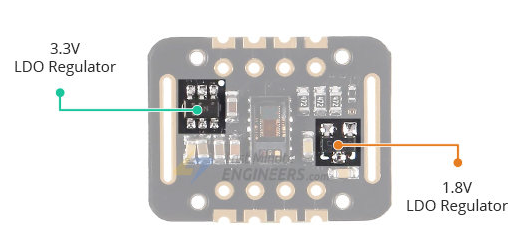
\includegraphics{chapitres/images/Capteur3.PNG}
		\label{fig:labelname}
	\end{figure}
	À l’arrière du circuit imprimé, vous trouverez un cavalier de soudure qui peut être utilisé pour sélectionner entre le niveau logique 3.3V et 1.8V. Par défaut, le niveau logique 3.3V est sélectionné, ce qui est compatible avec les niveaux logiques pour Arduino. Mais vous pouvez également sélectionner le niveau logique 1.8V selon vos besoins. Cela vous permet de connecter le module à n’importe quel microcontrôleur avec des E/S de niveau 5V, 3,3 V et même 1,8 V.
	\begin{figure}[h]
		\centering
		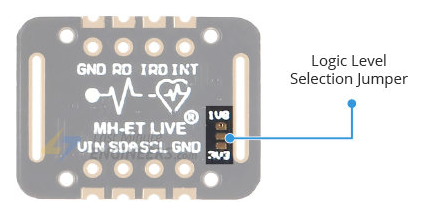
\includegraphics{chapitres/images/Capteur4.PNG}
		\label{fig:labelname}
	\end{figure}
	L’une des caractéristiques les plus importantes du MAX30102 est sa faible consommation d’énergie : le MAX30102 consomme moins de 600 uA pendant la mesure. Il est également possible de mettre le MAX30102 en mode veille, où il ne consomme que 0,7 uA. Cette faible consommation d’énergie permet une mise en œuvre dans des appareils alimentés par batterie tels que les combinés, les appareils portables ou les montres intelligentes.\newpage
	\begin{itemize}
		\item {\Large Comment fonctionnent l’oxymètre de pouls MAX30102 et le capteur de fréquence cardiaque?}
	\end{itemize}
	Le MAX30102, ou tout oxymètre optique de pouls et capteur de fréquence cardiaque d’ailleurs, se compose d’une paire de LED de haute intensité (RED et IR, toutes deux de longueurs d’onde différentes) et d’un photodétecteur. Les longueurs d’onde de ces LED sont respectivement de 660 nm et 880 nm.\newline
	\begin{figure}[h]
		\centering
		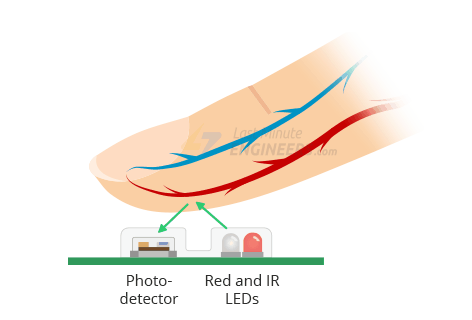
\includegraphics{chapitres/images/Capteur5.PNG}
		\label{fig:labelname}
	\end{figure}
	Le MAX30102 fonctionne en projetant les deux lumières sur le doigt ou le lobe de l’oreille (ou pratiquement partout où la peau n’est pas trop épaisse, de sorte que les deux lumières peuvent facilement pénétrer dans le tissu) et en mesurant la quantité de lumière réfléchie à l’aide d’un photodétecteur. Cette méthode de détection d’impulsions par la lumière est appelée photopléthysmogramme.

	Le fonctionnement du MAX30102 peut être divisé en deux parties: la mesure de la fréquence cardiaque et l’oxymétrie de pouls (mesure du niveau d’oxygène du sang).\newline
		\begin{itemize}
		\item {\Large Mesure de la fréquence cardiaque :}
    	\end{itemize}
		
	L’hémoglobine oxygénée (HbO2) dans le sang artériel a la caractéristique d’absorber la lumière IR. Plus le sang est rouge (plus l’hémoglobine est élevée), plus la lumière IR est absorbée. Lorsque le sang est pompé à travers le doigt à chaque battement de cœur, la quantité de lumière réfléchie change, créant une forme d’onde changeante à la sortie du photodétecteur. Au fur et à mesure que vous continuez à faire briller la lumière et à prendre des lectures de photodétecteurs, vous commencez rapidement à obtenir une lecture du pouls du rythme cardiaque (HR).
	\begin{figure}[h]
		\centering
		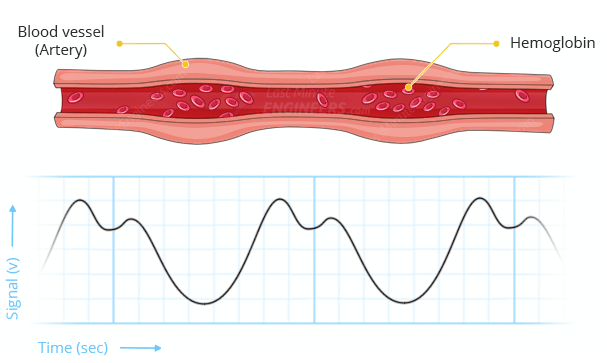
\includegraphics{chapitres/images/Capteur6.PNG}
		\label{fig:labelname}
	\end{figure}
	\begin{itemize}
		\item {\Large Oxymétrie de pouls :}
	\end{itemize}
	L’oxymétrie de pouls est basée sur le principe que la quantité de lumière ROUGE et IR absorbée varie en fonction de la quantité d’oxygène dans votre sang. Le graphique suivant représente le spectre d’absorption de l’hémoglobine oxygénée (HbO2) et de l’hémoglobine désoxygénée (Hb).
	\begin{figure}[h]
		\centering
		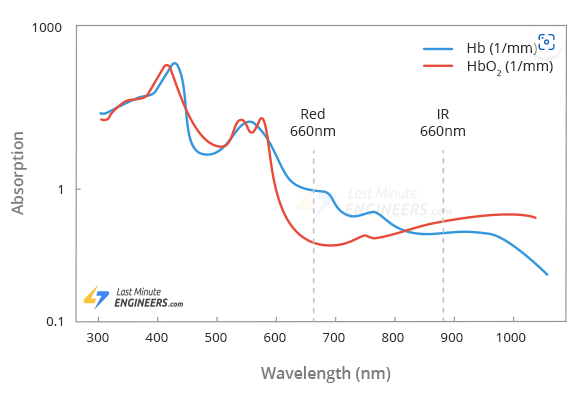
\includegraphics{chapitres/images/Capteur7.PNG}
		\label{fig:labelname}
	\end{figure}
	Comme vous pouvez le voir sur le graphique, le sang désoxygéné absorbe plus de lumière ROUGE (660 nm), tandis que le sang oxygéné absorbe plus de lumière IR (880 nm). En mesurant le rapport entre la lumière IR et la lumière ROUGE reçue par le photodétecteur, le niveau d’oxygène (SpO2) dans le sang est calculé.
	
	\subsection{\textcolor{green}{SSD1306 OLED display :}}
	L’écran SSD1306 contient une puce driver du même nom (SSD1306), il peut communiquer avec le périphérique maître (microcontrôleur, microprocesseur...) via le protocole I2C, le protocole SPI ou le protocole parallèle 8 bits. Dans cette rubrique, je vais montrer comment utiliser les protocoles I2C et SPI avec cet écran.
	Le protocole I2C n’a besoin que de 2 lignes: SDA (données série) et SCK (horloge série), une ligne supplémentaire est nécessaire qui est une ligne de réinitialisation (RST). Le protocole SPI est plus rapide que le protocole I2C mais il utilise plus de broches : SCK, SDA, CS (chip select : active low), D/C (data/command) et une broche de repos (RST).
	
	Le SSD1306 OLED que j'ai utilisé est montré ci-dessous (vue arrière), le mode par défaut est SPI qui peut être changé en I2C en retirant les résistances R3 et en plaçant les résistances R1 et R8 (comme écrit sur la carte). Notez que la résistance de R1 = R3 = R8 = 0 ohm.
		\begin{figure}[h]
			\centering
			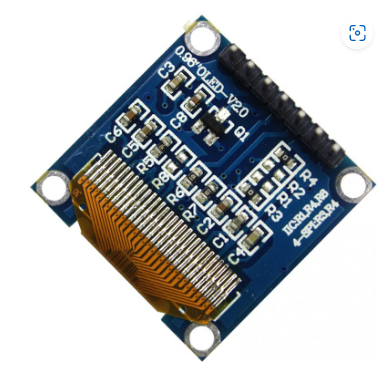
\includegraphics{chapitres/images/oled.PNG}
			\caption{L'écran SSD1306}
			\label{fig:labelname}
		\end{figure}
	\subsection{\textcolor{green}{AWS IOT core plateforme :}}
	
	AWS IoT Core est une plateforme cloud fournie par Amazon Web Services qui permet aux appareils de se connecter de manière sécurisée au cloud et d'interagir avec d'autres appareils et services. Elle fournit un ensemble de services gérés pour la création d'applications IoT, tels que l'enregistrement d'appareils, la communication sécurisée et le traitement de données.\newline
	
	Avec AWS IoT Core, vous pouvez connecter de manière sécurisée une large gamme d'appareils tels que des capteurs, des caméras et des appareils électroménagers au cloud et effectuer des actions sur les données qu'ils génèrent. Vous pouvez utiliser AWS IoT Core pour envoyer des commandes aux appareils, recevoir des données de ces derniers, et analyser et traiter les données en temps réel.\newline
	
	AWS IoT Core prend en charge différents protocoles IoT, notamment MQTT, HTTP et WebSockets, et fournit un ensemble de SDK et d'API pour faciliter l'intégration de vos appareils avec la plateforme. Elle propose également une intégration avec d'autres services AWS tels que AWS Lambda, Amazon Kinesis et Amazon S3 pour le traitement et le stockage de données.\newline
	
	Dans l'ensemble, AWS IoT Core fournit une plateforme évolutive et sécurisée pour la création d'applications IoT, vous permettant de créer, déployer et gérer rapidement et facilement des solutions IoT.
	\begin{figure}[h]
		\centering
		
\includegraphics{chapitres/images/aws.PNG}
		\caption{AWS IOT core plateforme}
		\label{fig:labelname}
	\end{figure}
	\subsection{\textcolor{green}{Conclusion :}}
	L'ESP8266 est un module Wi-Fi très populaire qui peut être utilisé pour connecter des dispositifs électroniques à Internet. Il est équipé d'un microcontrôleur et peut être programmé à l'aide de diverses langues de programmation telles que Lua et Python. Il est également compatible avec l'IDE Arduino.\newline
	
	L'oxymètre de pouls MAX30102 est un capteur optique de fréquence cardiaque et d'oxygène dans le sang intégré dans un seul module. Il utilise la technologie de photopléthysmographie (PPG) pour mesurer la fréquence cardiaque et la saturation en oxygène du sang. Il dispose également d'un amplificateur de photodiode intégré pour améliorer la précision des mesures.\newline
	
	AWS IoT Core est une plateforme cloud fournie par Amazon Web Services pour la création d'applications IoT. Elle permet aux appareils de se connecter de manière sécurisée au cloud et d'interagir avec d'autres appareils et services. AWS IoT Core prend en charge différents protocoles IoT et fournit un ensemble de services gérés tels que l'enregistrement d'appareils, la communication sécurisée, le traitement de données, ainsi qu'une intégration avec d'autres services AWS pour le stockage et le traitement de données. En résumé, AWS IoT Core fournit une plateforme évolutive et sécurisée pour la création, le déploiement et la gestion de solutions IoT.\newline
	

	\newpage
\end{flushleft}